\chapter{Case Study 1: An Aspect-Oriented Language}

\section{Introduction}

This chapter presents a metamodel for a simple aspect-oriented
language (AOL). We construct an abstract syntax model for the
language, along with an operational semantics and a concrete
syntax definition.

\section{AOL}

The AOL enables different aspects of components to be modelled
separately from the component itself, thus facilitating the
separation of concerns. The AOL is a general purpose language
because it can be applied across multiple languages provided that
they can access its metamodel. An example of its syntax is shown
below:

\begin{lstlisting}
@Aspect <name>
  ...
  @Class <path>
     <namedelement>
     ...
  end
end
\end{lstlisting}The aspect named $<$name$>$ adds one or more named elements to the
class referenced by the path $<$path$>$. In the version of AOL
presented here, classes are the components that aspects are added
to, but in practice any element can be viewed as a component.

As an example, consider the requirement to extend the class Box
with the ability to generate SVG (Scalable Vector Graphics).
Rather than merging this information into the class definition, an
aspect can be used to separate out this additional capability:

\begin{lstlisting}
@Aspect ToSVG
  @Class Box
    @Operation toSVG(parentx,parenty,out)
      if self.shown() then
        format(out,"<rect x=\"~S\" y=\"~S\" width=\"~S\" height=\"~S\"
        fill =\"#DBD5D5\" stroke=\"black\" stroke-width=\"1\"/>~\%",
        Seq{parentx+x,parenty+y,width,height});
        @For display in displays do
          display.toSVG(parentx+x,parenty+y,out)
        end
      end
    end
  end
\end{lstlisting}It is important to note that this is a much simpler mechanism than
that used by aspect-oriented programming languages such as
AspectJ. Nevertheless, it is still a useful and practical
mechanism for separating out different aspects of a model.

\section{Language Definition Strategy}

The approach taken to defining the syntax and semantics of this
language is to clearly separate syntax concepts from semantic
concepts. Parsing the concrete syntax for AOL results in an
intermediate abstract syntax definition, which is then desugared
into a model of the AOL's operational semantics.

\section{Abstract Syntax}

\subsection{Identification of Concepts}

Based on the example shown above the following candidates for
concepts can be immediately identified:

\begin{description}
\item [Aspect]  An aspect has a name and contains a collection of
components.

\item [Class] A class is a syntax concept that has a path to the
class that the named element is to be added to. A class is also a
component.

\item [NamedElement] The element that is added to the class
referenced by its path.
\end{description}

\subsection{Abstract Syntax Model}

An extended abstract syntax model is shown in figure
\ref{aspectabs2}.

\begin{figure}[htb]
\begin{center}
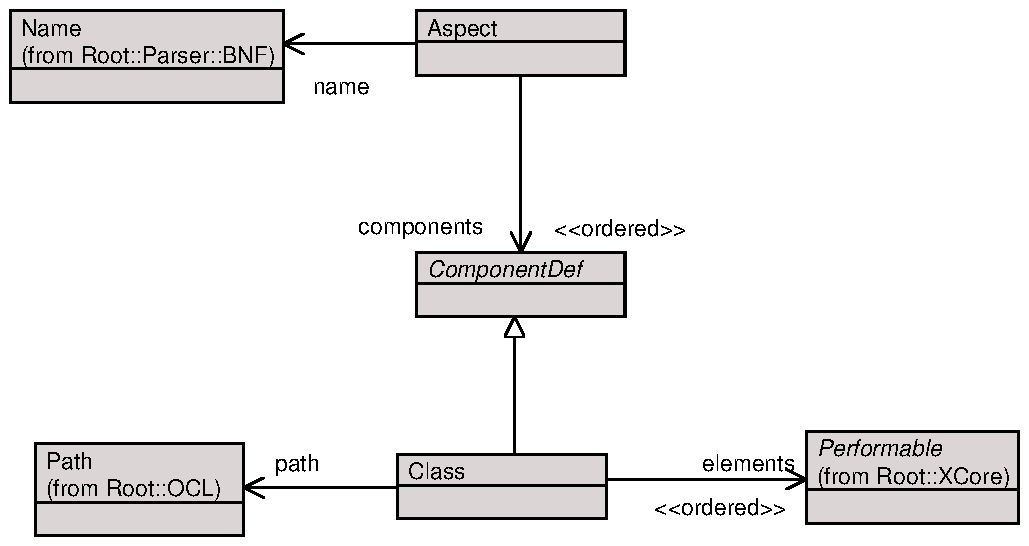
\includegraphics[width=14cm]{CaseStudy1/figures/abs2.pdf}
\caption{An abstract syntax model for AOL} \label{aspectabs2}
\end{center}
\end{figure}

There are a number of points to note about the model:

\begin{itemize}
\item Aspects have a name and are containers of component
definitions. A component definition is the abstract superclass of
all aspect component definitions  \item Class specialises
component and has a path to the class that its elements are to be
added to. The elements of Class are of type Performable (the Root
class for all parsable elements). \item Class is not the class
XCore::Class, but is purely a syntactical concept.
\end{itemize}

\section{Semantics}

The abstract syntax model focuses purely on syntax and does not
define a semantics. This is important for the AOL because there is
a clear separation between the language's syntax and the result of
parsing the syntax, which is to add a new named element to an
existing class.

To specify the semantics of the language we must therefore build a
semantic model. This is presented in figure \ref{aspectsem}.

\begin{figure}[htb]
\begin{center}
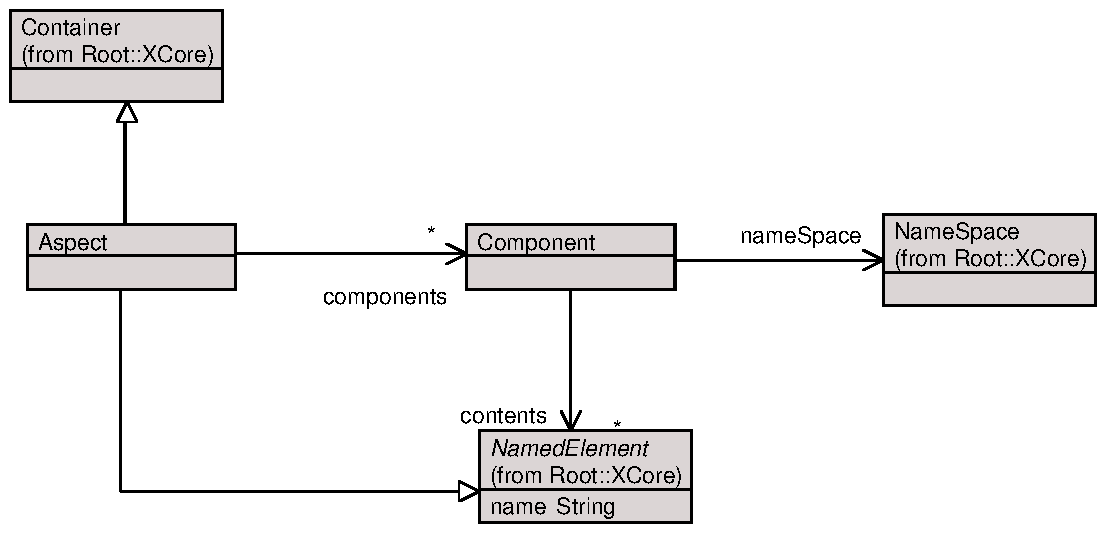
\includegraphics[width=14cm]{CaseStudy1/figures/semantics.pdf}
\caption{A semantic model for the AOL} \label{aspectsem}
\end{center}
\end{figure}

A component has a namespace and a collection of named elements
that are to be added to the namespace.

The following operation is required in order to add elements to a
component:

\begin{lstlisting}
context Component
  @Operation add(e:NamedElement)
    self.contents := contents->including(e)
  end
\end{lstlisting}The semantics of adding a named element to the namespace
referenced by the component is defined by the following operation:

\begin{lstlisting}
context Component
  @Operation perform()
    @For e in self.contents do
      nameSpace.add(e)
    end
  end
\end{lstlisting}\section{Concrete Syntax}

A concrete syntax for the AOL is defined in XBNF as follows. An
aspect is a name followed by a sequence of component definitions.
The result of parsing an aspect is to create an instance of the
abstract syntax class Aspect.

\begin{lstlisting}
  Aspect ::= name = Name components = (ComponentDef)* { Aspect(name,components) }.
\end{lstlisting}An aspect is then desugered into an instance of the semantics
class Aspect:

\begin{lstlisting}
  context Aspect
    @Operation desugar()
      components->iterate(c e = [| Aspects::Semantics::Aspect(<StrExp(name)>) |] | [| <e>.add(<c>) |])
    end
\end{lstlisting}An abstract syntax class definition is a path followed by a
sequence of expressions, which are the result of parsing the
elements that are to be added to the class:

\begin{lstlisting}
  Class ::= path = Path elements = Exp* { Class(path,elements) }.
  Path ::= root = VarExp names = ('::' Name)* { Path(root,names) }.
\end{lstlisting}Desugaring an abstract syntax class creates an instance of the
class Semantics::Component whose namespace is the class given by
the path of the syntax class, and whose elements are the named
elements of the abstract syntax class:

\begin{lstlisting}
  context Class
    @Operation desugar()
      elements->iterate(c e = [| Aspects::Semantics::Component(<path>) |] | [| <e>.add(<c>) |])
    end
\end{lstlisting}Once the desugaring process has occurred, the perform() operation
will be run on each component to add the named elements to the
class referenced by its path.

\section{Conclusion}

This chapter has shown that the key features of a simple
aspect-oriented language can be captured within metamodels. The
strategy taken was to keep the abstract syntax and semantic models
separate and use the concrete syntax definition to firstly create
an instance of the abstract syntax model, and then desugar it into
an instance of the semantic model.
